\documentclass[margin=0.1in]{standalone}
\usepackage{tikz}
\usepackage{amsfonts}
\usepackage{amsmath}
\begin{document}

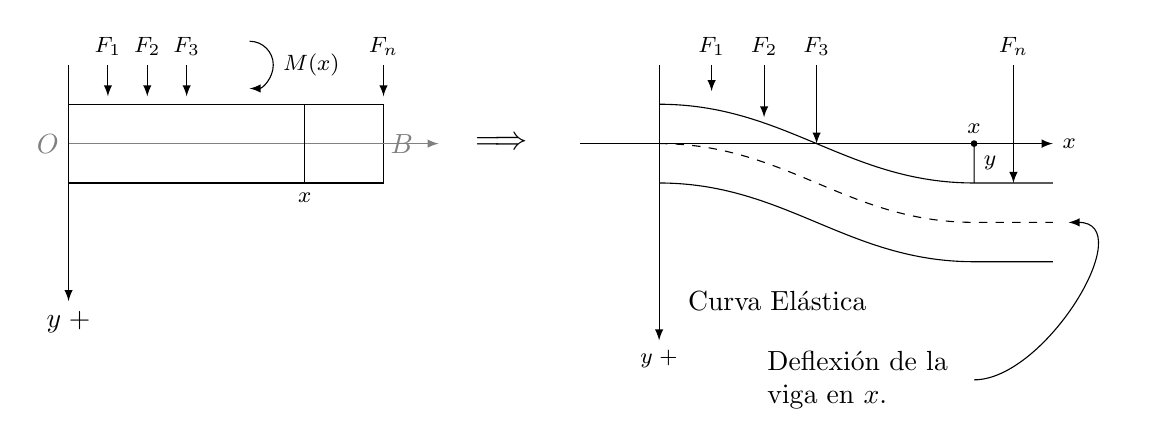
\begin{tikzpicture}[>=latex]
	\draw [->] (0,1) --++ (0,-3) node [below] {\(y\;+\)};
	\draw (0,0.5) rectangle (4,-0.5);
	\draw [gray,->] (0,0) node [left] {\(O\)} -- (4.7,0) node [left=2mm] {\(B\)};
	\foreach \n in {1,2,3} \draw [->] (\n/2,1) node [above] {\footnotesize \(F_\n\)} --++ (0,-0.4);
	\draw [->] (8/2,1) node [above] {\footnotesize \(F_n\)} --++ (0,-0.4);
	\draw (3,-0.5) node [below] {\footnotesize \(x\)} --++ (0,1);
	\draw [->] (2.3,1.3) arc (90:-90:3mm) node [midway, right] {\footnotesize \(M(x)\)};
	\node at (5.5,0) {\large \(\;\implies\;\)};
	\begin{scope}[xshift=7.5cm]
		\draw [->] (-1,0) -- (5,0) node [right] {\footnotesize \(x\)};
		\draw [->] (0,1) -- (0,-2.5) node [below] {\footnotesize \(y\;+\)};
		\draw (0,0.5) to [out=0 , in=180] (4,-0.5) --++ (1,0);
		\draw [dashed] (0,0) to [out=0 , in=180] (4,-1) --++ (1,0);
		\draw (0,-0.5) to [out=0 , in=180] (4,-1.5) --++ (1,0);
		\foreach \n in {1,2,3} \draw [->] (\n/1.5,1) node [above] {\footnotesize \(F_\n\)} --++ (0,-\n/3);
		\draw [->] (4.5,1) node [above] {\footnotesize \(F_n\)} --++ (0,-1.5);
		\filldraw (4,0) circle (1pt) node [above] {\footnotesize \(x\)} to node [right ,midway] {\footnotesize \(y\)} ++ (0,-0.5);
		\node at (1.5,-2) {Curva Elástica};
		\draw [->] (4,-3) node [left, text width=2.5cm] {Deflexión de la viga en \(x\).} to [out = 0, in=0]  (5.2,-1);
	\end{scope}
\end{tikzpicture}

\end{document}
